\chapter{引\hspace{1em}言}

本模板的面向对象不包括对\LaTeX 知识完全不了解之人,特别不适合%
不愿付出适当时间来学习\LaTeX 知识的人。如果您是\LaTeX 新手,本人%
推荐您阅读一些入门文档,比如“lshort”,该文档有社区翻译的中文版本%
《一份不太简短的\LaTeXe 介绍》,您可以从互联网很轻松的找到该文件。%
如果您更加愿意阅读书籍来获得相应的知识,常见的中文书籍有%
陈志杰等\scite{陈志杰LaTeX}编写的《\LaTeX 入门与提高》,但该书涉及%
的知识部分已经过时,且该书作者年纪已大,所以该书也不会继续更新了。%
值得推荐的入门书籍是由刘海洋\scite{刘海洋LaTeX}编写的《\LaTeX 入门》,%
该书作者(LeoLiu)活跃于\CTeX 论坛,是主要板块的版主,同时刘海洋在知乎上%
关于\LaTeX 知识也有许多值得参考的回答,该书的好处是可以让你快速了解必须%
的\LaTeX 知识,同时拓展视野。若您对\LaTeX 知识已有了解,但是涉及不深,%
本人推荐您阅读胡伟\scite{胡伟LaTeX}编写的《\LaTeXe 完全学习手册》,该书%
对常见的\LaTeX 知识做了比较全面的总结,对一些常见的宏包也有介绍,是一本%
不错的工具书籍,可供随时查阅。如果您的\LaTeX 水平已经相当高了,这部分介绍%
可以完全忽略之。如果您问\LaTeX 知识仅止于此吗?答案显然是否定的。例如,%
《The \LaTeX Companion》一书介绍了许多宏包的使用,\TeX 系统作者的书籍%
《The \TeX\ Book》等介绍了更初级的\TeX 命令等。\LaTeX 知识尤其是\TeX 知识%
有时候总是令人困惑的,例如\TeX 中命令的展开方式和时机等,本人疑惑得早已放弃治疗了,%
希望\LaTeX3正式版可以早日推出,让这些事情变得更加简单。

\begin{figure}[h]
  \centering
  % Requires \usepackage{graphicx}
  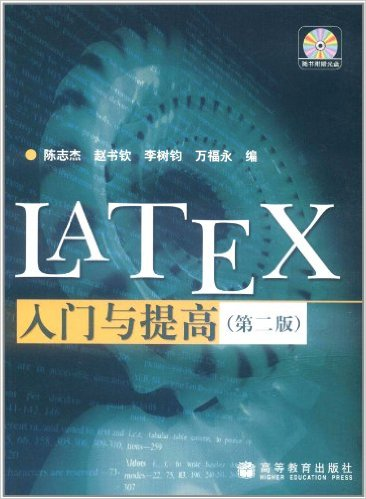
\includegraphics[width=0.2\textwidth]{pic/book/ChenZhiJie.jpg} \quad
  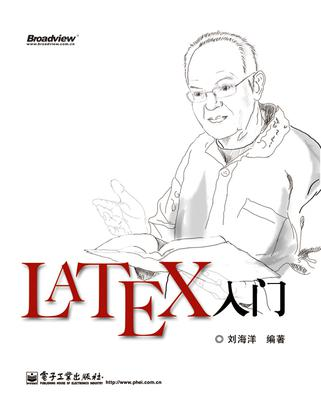
\includegraphics[width=0.2\textwidth]{pic/book/LiuHaiYang.jpg} \quad
  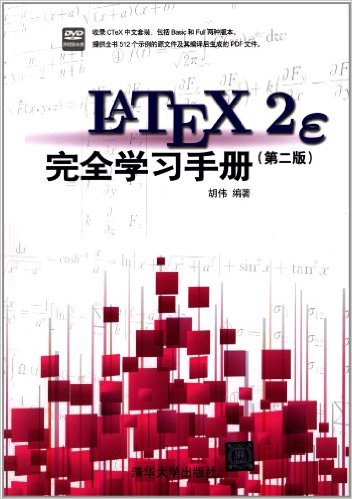
\includegraphics[width=0.2\textwidth]{pic/book/HuWei.jpg}   \quad
  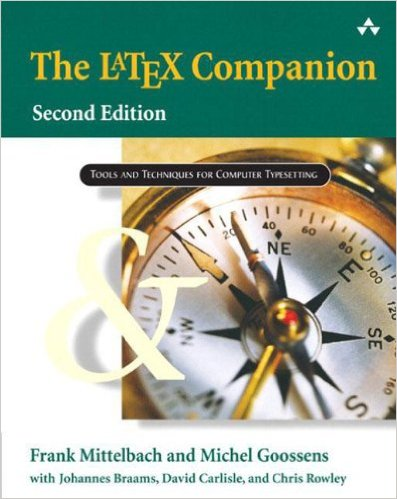
\includegraphics[width=0.2\textwidth]{pic/book/LaTeXCompanion.jpg}
  \caption{\LaTeX 中英文书籍}
\end{figure}

关于本模板的使用,\textbf{您需要的\LaTeX 知识相当少},本文接下来会一一介绍如何使用之。%


\section{软件环境}
\subsection{软件安装}
本文只针对Windows环境,至于Linux环境,本人默认Linux用户能够轻松配置使用之。%
为了快速上手,许多人会选择安装\CTeX 套装,该套装在%
\url{http://www.ctex.org/CTeXDownload} 页面下载,请选择安装%
CTeX\_2.9.2.164\_Full.exe (1.31G)版本,虽然该套装已停止更新,%
但是我们可以通过该套装自带的包更新器更新相应的宏包,而且即使不联网更新,%
该版本也已基本涵盖了我们常用的宏包。%
在这里,本人还是推荐您安装TeXLive,%
该套装的宏包通常比较新。本模板在TeXLive 2015下编译完成,%
本人不保证其在\CTeX 套装的兼容性。接下来,本人假设您已经安装好了以上其中一个版本。%


\subsection{编辑器}
这里采用\CTeX 套装默认的WinEdt,该编辑器专门针对\LaTeX,如果您安装了\CTeX 套装,那么%
该编辑器已经安装好了。如果使用的是TeXLive,那么也可以另外下载该编辑器安装,%
虽然WinEdt是付费软件,但是\dots,没有但是。%
关于更多编辑器的介绍,例如Vim等,您可以去维基百科或者知乎上搜索,有许多%
相应的介绍。关于WinEdt的基本配置和使用,请您阅读本模板附带的图文说明文档%
《第一次使用LaTeX?读我》。接下来,本人默认您已经基本熟悉WinEdt的使用了。


\section{注意事项}
\begin{itemize}
  \item \textbf{本模板的放置路径不含中文或其他乱码字符。}原因是使用Biber编译参考文献时,%
  需要用到管理员权限,而一键编译的脚本,在转换工作路径时,如果含有例如中文,%
  会导致无法正确转换。总而言之,您就用英文就万事大吉了,例如本人的放置路径为:\\
  \verb"F:\WorkDocument\CARDC-Thesis-LaTeX-Template"。

  \item \textbf{图片等资源的文件名请使用英文},确保没有惊喜。
\end{itemize}

\section{问题反馈}
虽然被人已经尽力测试,但是仍不免有不足之处,如果发现有何问题,可以向本人反馈。
